\section{Background: Long CoT Reasoning Models and the Overthinking Phenomenon}

\subsection{Chain-of-Thought (CoT) Reasoning}

Chain-of-Thought (CoT) reasoning~\cite{wei2022chain} is a key approach that has been purposefully introduced in LLMs to enhance their reasoning capabilities. In this setting, models are typically prompted to generate a structured reasoning chain before arriving at a final answer. Techniques in this domain have been shown to improve overall accuracy~\cite{wei2022chain} since a higher-quality generation context often leads to more consistent and reliable final results. Several notable CoT variants have been developed: Self-Consistency CoT~\cite{wang2023self} replaces the standard greedy decoding approach by sampling diverse reasoning paths and selecting the most consistent answer through marginalization and aggregation. Tree-of-Thought (ToT) prompting~\cite{yao2023tree} further structures the reasoning process as a tree with backtracking, significantly improving efficiency in solving parallelizable subtasks. Graph-of-Thoughts (GoT) prompting~\cite{besta2024graph} extends this concept by structuring thoughts into a graph, allowing iterative refinement of individual reasoning steps. While many CoT variants exist, they generally involve different prompting techniques to guide the behavior of models, sometimes incorporating controller-like mechanisms to manage thought progression and usage.

\subsection{The Mechanism Behind Large Reasoning Models}

Multi-step reasoning refers to the ability of LLMs ability to generate structured reasoning steps before committing to a final answer. This capability is particularly beneficial for logic-intensive tasks such as mathematics and programming. More broadly, reasoning-capable models are often favored by human users over their non-reasoning counterparts, as evidenced by rankings in the Chatbot Arena LLM Leaderboard.\footnote{A community-driven evaluation of leading LLMs and AI chatbots: \url{https://lmarena.ai/?leaderboard}.}

Recent reasoning models, such as DeepSeek-R1~\cite{guo2025deepseek} and OpenAI o1~\cite{luo2025o1}, are known or believed to have internalized reasoning behaviors, reducing reliance on explicit test-time augmentations. These models generate detailed CoT reasoning by iteratively producing intermediate steps and refining solutions sequentially until reaching a final answer. Unlike traditional CoT approaches, which rely on prompting, these reasoning models internalize their reasoning capability through extensive training.

The OpenAI o1 model is speculated to employ a tree-based search approach, such as Monte Carlo Tree Search (MCTS)~\cite{kocsis2006bandit, coulom2006efficient}, combined with a Process Reward Model (PRM) to explore reasoning paths and determine optimal solutions through guided simulations.\footnote{There is no official confirmation regarding OpenAI o1’s training details and mechanisms. However, sources such as \url{https://www.interconnects.ai/p/openais-o1-using-search-was-a-psyop} and \url{https://www.youtube.com/watch?v=6PEJ96k1kiw} discuss these speculations in detail and are recommended for interested readers.} DeepSeek-R1, on the other hand, explicitly learns its reasoning capability through supervised fine-tuning and reinforcement learning, with a particular emphasis on rule-based rewards for math and coding tasks. These models are trained to generate reasoning steps in a predefined format before arriving at their final answers.

\subsection{The Overthinking Problem in Long CoT Reasoning Models}

\begin{figure}[t]
    \centering
    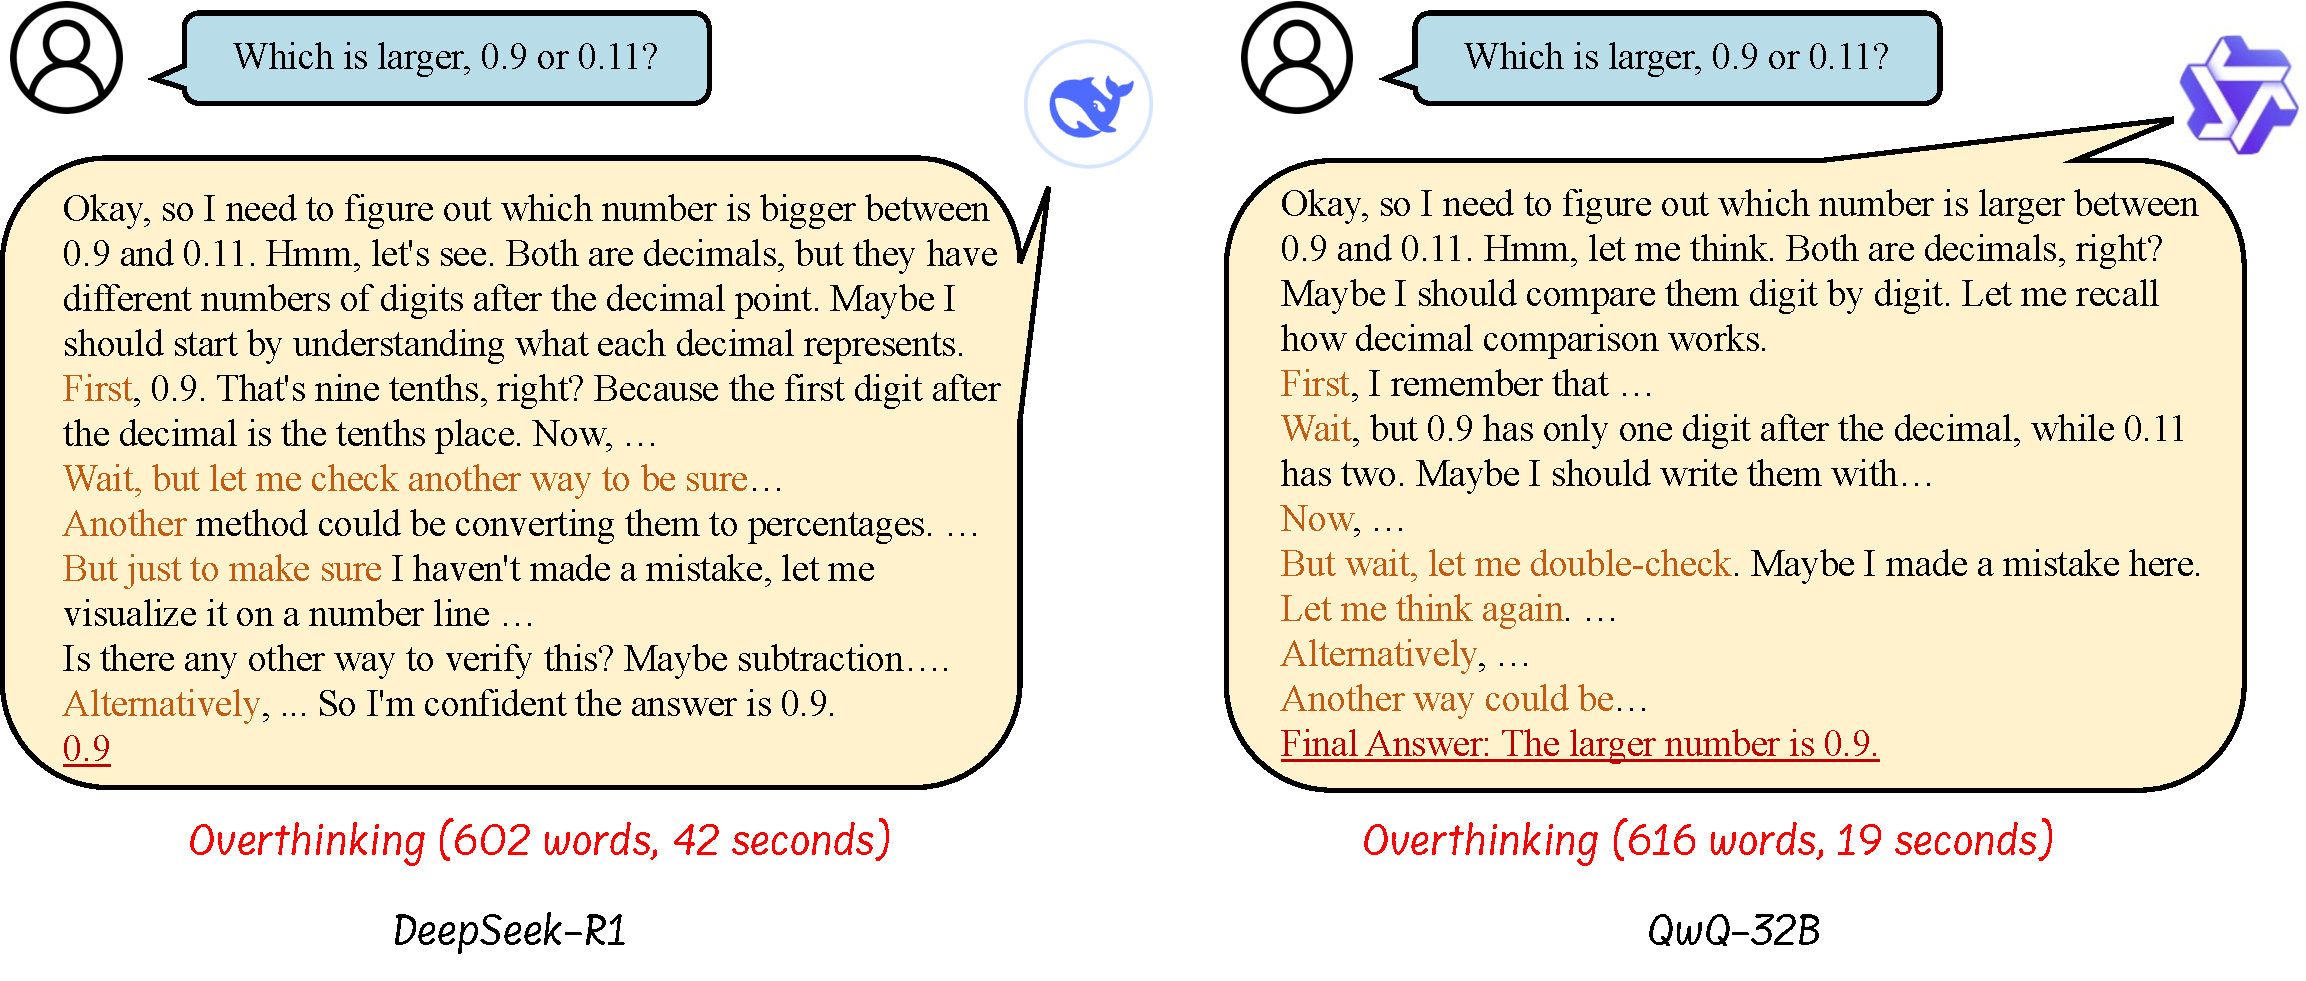
\includegraphics[width=0.99\linewidth]{figs/overthinking.pdf}
    \caption{An example of the ``overthinking phenomenon'': when asked \textbf{\textit{``Which is larger, 0.9 or 0.11?''}}, the reasoning model takes an unnecessarily long time (e.g., 19 seconds for QwQ-32B~\cite{qwen_qwq_32b_preview} and 42 seconds for DeepSeek-R1~\cite{guo2025deepseek}) to arrive at the correct answer. This example was tested in March 2025.}
    \label{fig:overthink-generation}
\end{figure}

The ``overthinking phenomenon''~\cite{team2025kimi,chen2024not} in long CoT reasoning models refers to situations where LLMs generate excessively detailed or unnecessarily elaborate reasoning steps, ultimately reducing their problem-solving efficiency. In particular, many modern reasoning models, especially those with smaller parameter scales, tend to produce verbose reasoning or redundant intermediate steps, making them unable to provide answers within the user-defined token budget. In worse cases, excessive reasoning steps introduce errors or obscure logical clarity, leading to incorrect answers.

Figure~\ref{fig:overthink-generation} illustrates an example of overthinking. Even though the model arrives at the correct answer early in its reasoning process, it continues generating unnecessary intermediate steps, leading to inefficiencies. Given the substantial resource costs associated with LLM inference (e.g., OpenAI o1 costs \$60 per 1M generated tokens), such behavior is highly undesirable. Moreover, the problem becomes even worse if longer reasoning leads to wrong answers. In contrast, efficient reasoning models would use fewer reasoning steps to obtain correct answers while reducing inference costs.

Addressing this challenge is particularly difficult because the pretraining recipes for reasoning-capable models often explicitly encourage generating extended reasoning steps to improve accuracy. For example, DeepSeek-R1-Zero, a more or less a development prototype of DeepSeek-R1, exhibits a direct correlation between increased training duration with longer response lengths and improved benchmark performance~\cite{guo2025deepseek}. These trends are often viewed as proxies for successful reasoning training. Consequently, improving inference efficiency requires working against certain pretraining objectives, making it a non-trivial challenge. 

This paper aims to systematically summarize various approaches and methodologies toward achieving the challenging yet valuable goal of developing reasoning models with high efficiency and strong reasoning capabilities.
